\begin{figure}[H] 
\centering 
\includegraphics[width=1\textwidth]{docs/img/svg/Skeleton!Hide!Skeleton hide!SpaceShip hide when is hidden Com!SpaceShip hide when it is hidden_54.png} 
\caption{Egy űrjármű elbújik. A telepesek helyet foglalnak az aszteroidában, amikor elbújnak, ezért csak korlátozott számú telepes bújhat el.} 
\end{figure} 

\begin{figure}[H] 
\centering 
\includegraphics[width=1\textwidth]{docs/img/svg/Skeleton!Hide!Skeleton hide!SpaceShip hide when asteroid exploded Com!SpaceShip hide when asteroid e_55.png} 
\caption{Egy űrjármű elbújik. A telepesek helyet foglalnak az aszteroidában, amikor elbújnak, ezért csak korlátozott számú telepes bújhat el.} 
\end{figure} 

\begin{figure}[H] 
\centering 
\includegraphics[width=1\textwidth]{docs/img/svg/Skeleton!Hide!Skeleton hide!SpaceShip hide when core is invisible Com!SpaceShip hide when core is in_56.png} 
\caption{Egy űrjármű elbújik. A telepesek helyet foglalnak az aszteroidában, amikor elbújnak, ezért csak korlátozott számú telepes bújhat el.} 
\end{figure} 

\begin{figure}[H] 
\centering 
\includegraphics[width=1\textwidth]{docs/img/svg/Skeleton!Hide!Skeleton hide!SpaceShip hide when is able to hide Com!SpaceShip hide when is able to h_57.png} 
\caption{Egy űrjármű elbújik. A telepesek helyet foglalnak az aszteroidában, amikor elbújnak, ezért csak korlátozott számú telepes bújhat el.} 
\end{figure} 

\begin{figure}[H] 
\centering 
\includegraphics[width=1\textwidth]{docs/img/svg/Skeleton!Hide!Skeleton hide!SpaceShip exitHiding  when is not hidden Com!SpaceShip exitHiding  when _58.png} 
\caption{Egy űrjármű kijön a rejtekhelyéről.} 
\end{figure} 

\begin{figure}[H] 
\centering 
\includegraphics[width=1\textwidth]{docs/img/svg/Skeleton!Hide!Skeleton hide!SpaceShip exitHiding  when used space Com!SpaceShip exitHiding  when use_59.png} 
\caption{Egy űrjármű kijön a rejtekhelyéről.} 
\end{figure} 

\begin{figure}[H] 
\centering 
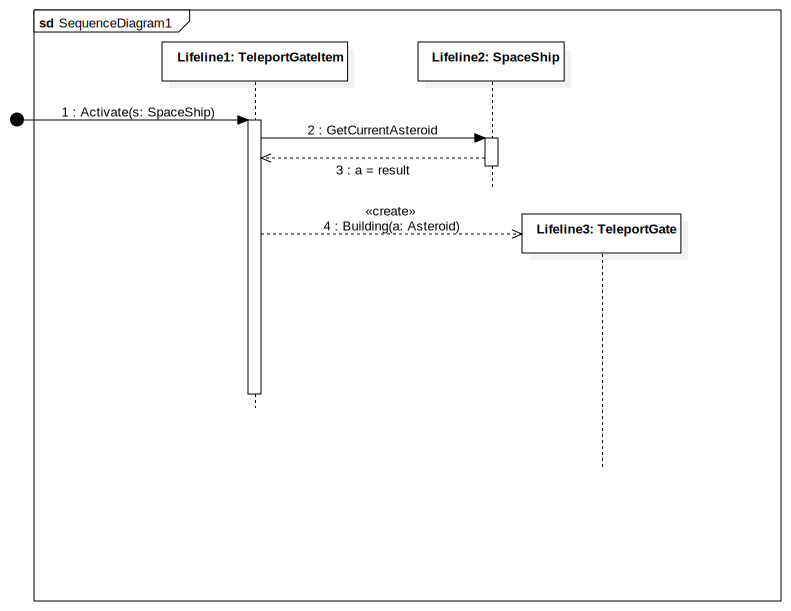
\includegraphics[width=1\textwidth]{docs/img/svg/Skeleton!Place gate!Interaction1!SequenceDiagram1_34.png} 
\caption{Test docs
} 
\end{figure} 

\begin{figure}[H] 
\centering 
\includegraphics[width=1\textwidth]{docs/img/svg/Skeleton!Drill!Skeleton drill!SpaceShip drill when asteroid exploded Com!SpaceShip drill when astero_45.png} 
\caption{Csak akkor tudunk mélyíteni a kérgen, ha nem robbant fel már az aszteroida és ha nem fúrtunk már át a lérgen.} 
\end{figure} 

\begin{figure}[H] 
\centering 
\includegraphics[width=1\textwidth]{docs/img/svg/Skeleton!Drill!Skeleton drill!SpaceShip drill when core is visible Com!SpaceShip drill when core is _46.png} 
\caption{Csak akkor tudunk mélyíteni a kérgen, ha nem robbant fel már az aszteroida és ha nem fúrtunk már át a lérgen.} 
\end{figure} 

\begin{figure}[H] 
\centering 
\includegraphics[width=1\textwidth]{docs/img/svg/Skeleton!Drill!Skeleton drill!SpaceShip drill when succeed Com!SpaceShip drill when succeed Com_47.png} 
\caption{Csak akkor tudunk mélyíteni a kérgen, ha nem robbant fel már az aszteroida és ha nem fúrtunk már át a lérgen.} 
\end{figure} 

\begin{figure}[H] 
\centering 
\includegraphics[width=1\textwidth]{docs/img/svg/Skeleton!Solar flare!Interaction1!Tester queues solar flare for nex round_34.png} 
\caption{A tesztelő be tudja állítani, hogy a kör végén legyen-e napkitörés.} 
\end{figure} 

\begin{figure}[H] 
\centering 
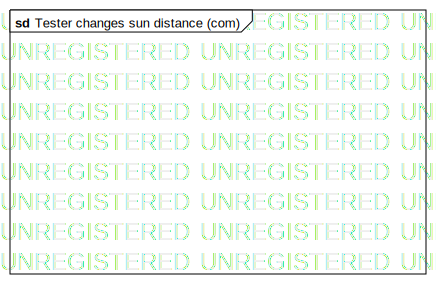
\includegraphics[width=1\textwidth]{docs/img/svg/Skeleton!Move asteroid field!Change Sun Distance!Communication!Tester changes sun distance (com)_37.png} 
\end{figure} 

\begin{figure}[H] 
\centering 
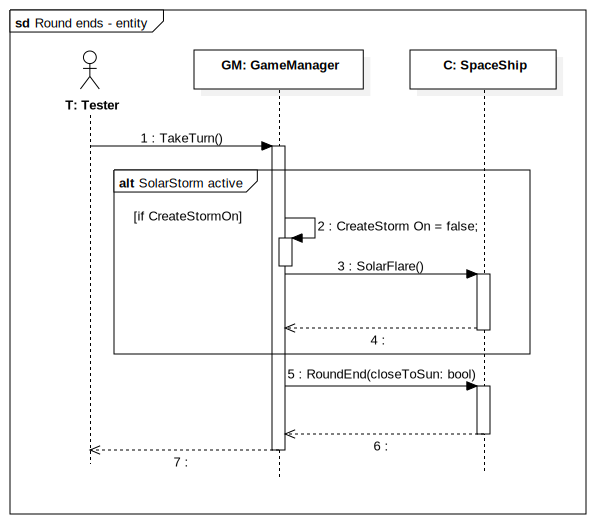
\includegraphics[width=1\textwidth]{docs/img/svg/Skeleton!Move asteroid field!Collaboration2!Sequence!Round ends - entity_39.png} 
\caption{Az űrjárműveken leken is meghívódik a RoundEnd függvény. Őket nem befolyásolja a napközelség.
Az aszteroidákat azonban igen, ők külön ábrázolva vannak!} 
\end{figure} 

\begin{figure}[H] 
\centering 
\includegraphics[width=1\textwidth]{docs/img/svg/Skeleton!Place resource!Skeleton placeResource!SpaceShip place resource when asteroid exploded Com!S_65.png} 
\caption{Lehelyezünk egy tárgyat az átfúrt kérgű, üreges aszteroidába.} 
\end{figure} 

\begin{figure}[H] 
\centering 
\includegraphics[width=1\textwidth]{docs/img/svg/Skeleton!Place resource!Skeleton placeResource!SpaceShip place resource when core is invisible Com!S_66.png} 
\caption{Lehelyezünk egy tárgyat az átfúrt kérgű, üreges aszteroidába.} 
\end{figure} 

\begin{figure}[H] 
\centering 
\includegraphics[width=1\textwidth]{docs/img/svg/Skeleton!Place resource!Skeleton placeResource!Place resource when core has resource Com!SpaceShip p_67.png} 
\caption{Lehelyezünk egy tárgyat az átfúrt kérgű, üreges aszteroidába.} 
\end{figure} 

\begin{figure}[H] 
\centering 
\includegraphics[width=1\textwidth]{docs/img/svg/Skeleton!Place resource!Skeleton placeResource!SpaceShip place resource when core is full Com!SpaceS_68.png} 
\caption{Lehelyezünk egy tárgyat az átfúrt kérgű, üreges aszteroidába.} 
\end{figure} 

\begin{figure}[H] 
\centering 
\includegraphics[width=1\textwidth]{docs/img/svg/Skeleton!Place resource!Skeleton placeResource!SpaceShip place resource when succeed Com!SpaceShip p_69.png} 
\caption{Lehelyezünk egy tárgyat az átfúrt kérgű, üreges aszteroidába.} 
\end{figure} 

